\section{Experimental results} \label{experiments}

\subsection{Dataset insights}  \label{ch:experimentsA}

This chapter presents the dataset insights of the complete dataset with full genome sequences and the dataset insights of the preprocessed dataset.

\subsubsection{Complete dataset}  \label{ch:experimentsAa}

\begin{wrapfigure}{R}{8cm}
	\centering
	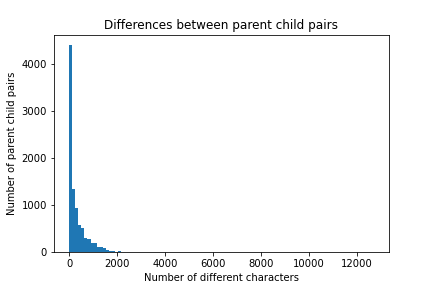
\includegraphics[width=0.9\linewidth]{figures/distributionDifferencesParentChild.png}
	\caption{Distribution of the differences between parent and child sequences \cite{own representation}}
	\label{distributionDifferencesParentChild}
\end{wrapfigure}

The dataset consists of 9199 parent-child pairs.
The distribution how the parent and child sequences differ can be seen in figure \ref{distributionDifferencesParentChild}. The majority of parent-child pairs differ in less than 200 characters. The number of completely equal parent-child pairs is 396.

\vspace{2cm}
Figure \ref{mutatedGeneticLoci} visualizes the distribution of mutations over the full \ac{SARS-CoV-2} genome.

\begin{figure}[ht!]
	\centering
	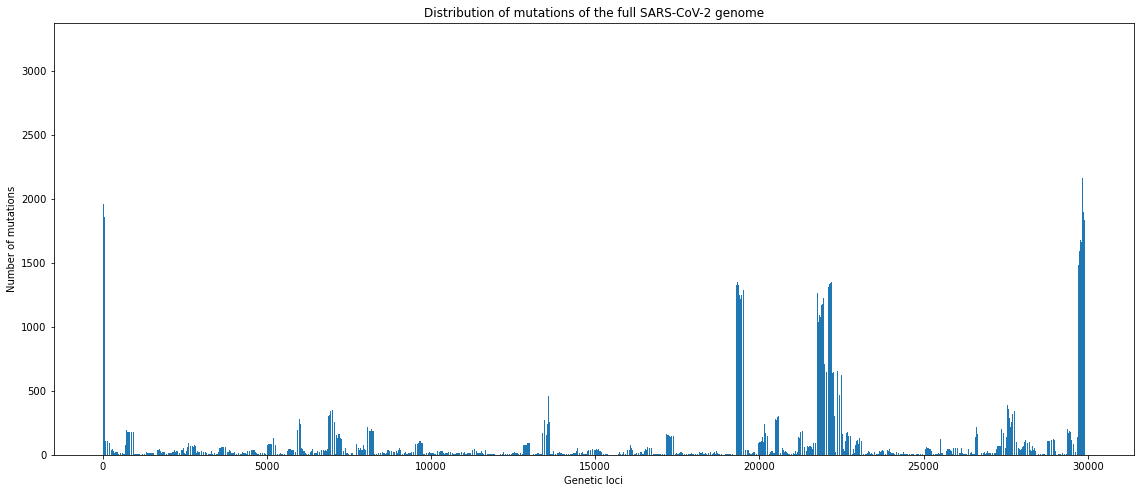
\includegraphics[width=1.0\linewidth]{figures/mutatedGeneticLoci.png}
	\caption{Mutated genetic loci \cite{own representation}}
	\label{mutatedGeneticLoci}
\end{figure}

\newpage
\subsubsection{Preprocessed dataset}  \label{ch:experimentsAb}

The complete dataset is preprocessed as described in chapter \ref{ch:approachB}. The distribution how the parent and child amino acids differ in the selected subpart can be seen in figure \ref{preprocessedDistributionDifferencesParentChild}. The majority (6946) of parent-child pairs are equal. This is not optimal for training the \ac{ML} model and is further discussed in chapter \ref{ch:experimentsB}. 

\begin{figure}[ht]
	\centering
	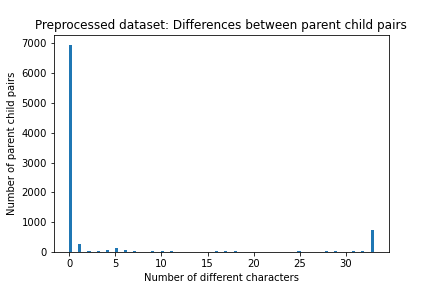
\includegraphics[width=0.6\linewidth]{figures/preprocessedDistributionDifferencesParentChild.png}
	\caption{Preprocessed dataset: Distribution of the differences between parent and child sequences \cite{own representation}}
	\label{preprocessedDistributionDifferencesParentChild}
\end{figure}

Figure \ref{preprocessedMutatedGeneticLoci} visualizes the differing amino acids and their positions of the selected subpart of the \ac{SARS-CoV-2} genome. They are distributed equally over the selected subpart.

\begin{figure}[ht]
	\centering
	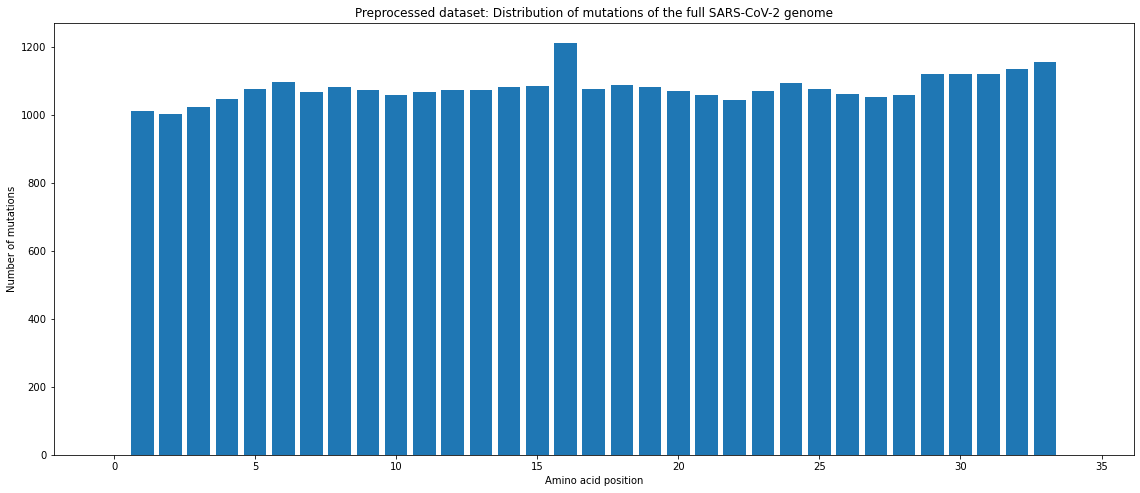
\includegraphics[width=0.9\linewidth]{figures/preprocessedMutatedGeneticLoci.png}
	\caption{Preprocessed dataset: Differing amino acid positions \cite{own representation}}
	\label{preprocessedMutatedGeneticLoci}
\end{figure}

\newpage
\subsection{Evaluation}  \label{ch:experimentsB}

\subsubsection{Evaluation criteria}

To measure the success of the transformer model different evaluation criteria need to be introduced that capture how well the mutations observed in the data can be reproduced by the generator. A mutation prediction is considered correct in case the prediction matches in codons and locations. Further to distinguish are partially correct mutation predictions in case mutations are observed at the right locations but in different codons. Mutation predictions can further be considered as wrong in case they were not observed in the true child sequences or missed in case they could not be observed in the generated sequences. 

A common metric used in the domain of \ac{NMT} is the so-called \ac{BLEU} score \cite{Papineni2002}. Its so-called modified n-gram precision captures common n-grams between the generated sentence and the true reference translation sentence independently of their position. Also a sentence brevity penalty is incorporated into the score. The \ac{BLEU} score ranges between zero and one with one being a perfect match to the reference translation. \cite{Papineni2002}

Using solely the \ac{BLEU} score would mean less focus on the concrete mutation prediction at critical genome positions but rather a correct overall child sequence prediction. As the child sequence is mostly similar to the parent sequence, predicting a nearly identical child sequence is not too difficult and the \ac{BLEU} score would resolves already to a high value at early stages of training. 

Therefore the MutaGAN paper \cite{Berman2020} introduced several other metrics besides the \ac{BLEU} score. For instance the distribution of specific codon mutations between the ground truth data and the generated data was calculated to evaluate the similarity of both mutation profiles. Furthermore a so-called sequence true positive rate is determined by capturing all observable mutations over all generated child sequences and comparing them to the list of actual existing mutations in the ground truth data. 

Besides the \ac{BLEU} score, we also utilize the sequence true positive rate to evaluate the model using Google's \textit{Diff Match and Patch} libraries to identify the mutations\footnote{For the Diff Match and Patch libraries, see \url{https://github.com/google/diff-match-patch}}. The Levenshtein distance is used as a simple metric to evaluate the degree of similarity between parent and generated child sequences. 

\subsubsection{Transformer pretraining}  \label{ch:experimentsBa}

Figure \ref{pretrainingLossPlot} shows the loss plot for the Transformer pretraining. The model converges rather fast. The first meaningful results are already reached after 2 epochs. The reached BLEU score is 0.8559. From this point of view the results look very promising. That is why the details of these results are investigated. When comparing all predictions with the true values it is noticeable, that the model prediction is always the same for all 460 test instances. This could be explained by the fact, that the predicted sequence is correct in 318 of 460 cases. Therefore it can be assumed, that the model works, but the used dataset is not optimal.

\begin{figure}[ht]
	\centering
	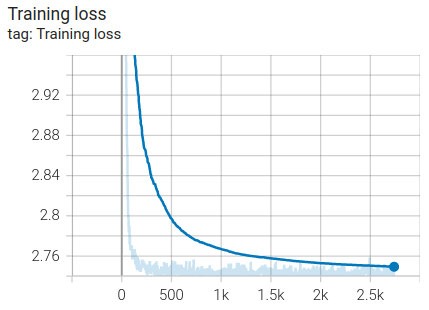
\includegraphics[width=0.5\linewidth]{figures/pretrainingLossPlot.png}
	\caption{Transformer pretraining loss plot}
	\label{pretrainingLossPlot}
\end{figure}


\subsubsection{GAN training}  \label{ch:experimentsBb}

TODO

\newpage
